% <- percent signs are used to comment
\documentclass[12pt]{article}

%%%%%% PACKAGES - this part loads additional material for LaTeX %%%%%%%%%
% Nearly anything you want can be done in LaTeX if you load the right package 
% (search ctan.org or google it if you are looking for something).  We will load
% here a few that we need for this document or that we expect you to need later.

% The next 3 lines are needed to fix shortcomings of TeX that only make sense given its 40-year history ...
% Simple keep and ignore.
\usepackage[utf8]{inputenc}
\usepackage[T1]{fontenc}
\usepackage{lmodern}
\usepackage{amsmath}
\usepackage{changepage}
\usepackage{lipsum}
\usepackage{bm}
\usepackage{ulem}


% Custom margins (and paper sizes etc.) because LaTeX else wastes much space
\usepackage[margin=1in]{geometry}

% The following packages are created by the American Mathematical Society (AMS)
% and provide lots of tools for special fonts, symbols, theorems, and proof
\usepackage{amsmath,amsfonts,amssymb,amsthm}
% mathtools contains many detail improvements over ams and core tex
\usepackage{mathtools}

% graphicx is required for images
\usepackage{graphicx}

% enumitem used for customizing enumerations
\usepackage[shortlabels]{enumitem}

% tikz is the package used for drawing, in particular for drawing trees. You may also find simplified packages like tikz-qtree and forest useful
\usepackage{tikz}

% hyperref allows links, urls, and many other PDF tricks.  We load it here
%          in such a way that the PDF file has info about it
\usepackage[%
	pdftitle={CS251 Assignment 0},%
	hidelinks,%
]{hyperref}


%%%%%% COMMANDS - here you can define your own LaTeX-commands %%%%%%%%%

%%%%%% End of Preamble %%%%%%%%%%%%%

\begin{document}

\begin{center}
{\Large\textbf{CS251, Spring 2022}}\\
\vspace{2mm}
{\Large\textbf{Assignment 2: Question 5}}\\
\vspace{3mm}
\end{center}
\begin{adjustwidth}{0em}{0pt}
\textbf{Q5a)} Design a Moore finite-state machine (where the input is X and the output is Z)cthat outputs 1 after the input is constant for 3 clock cycles, i.e. after 3 consecutive 1s, or 3 consecutive 0s. If the input changes again, the output goes back to 0 until the constant input condition is met again. Draw a fully labeled state diagram.\\
\begin{figure}[tbhp]
	\begin{center}
		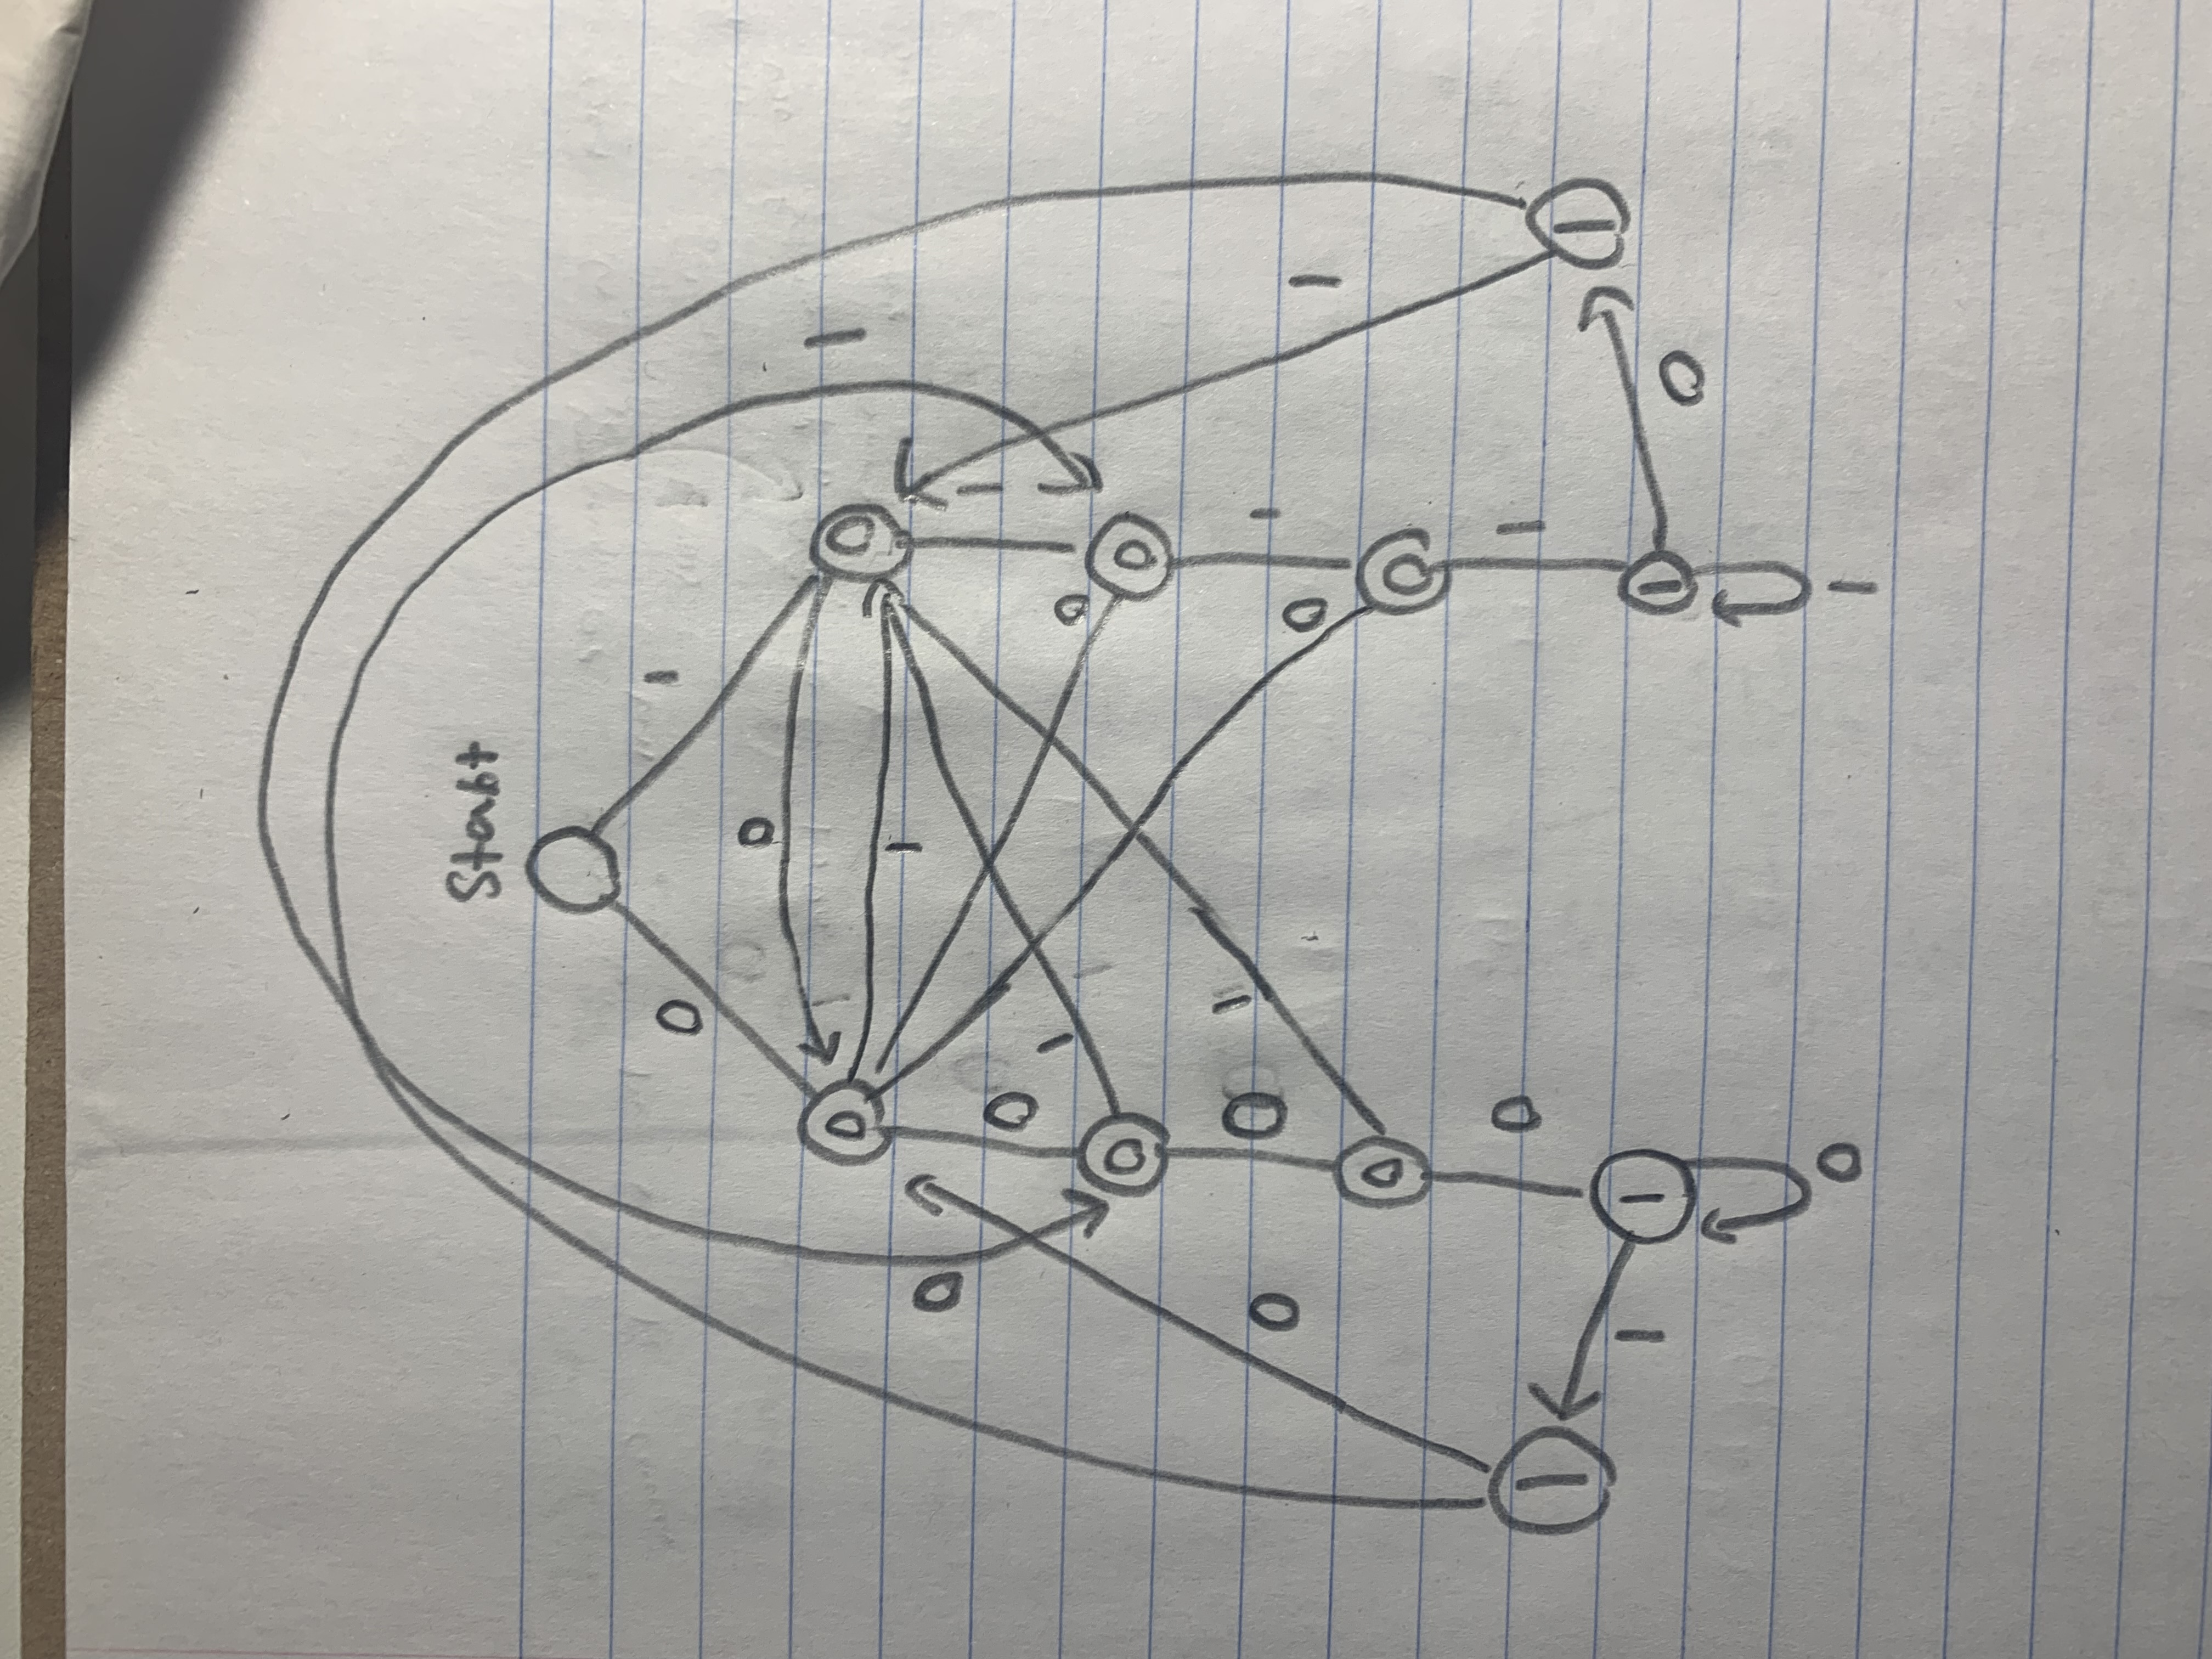
\includegraphics[width=1\textwidth, angle=270]{graph.jpg}
	\end{center}
\end{figure}

\end{adjustwidth}
\begin{adjustwidth}{0em}{0pt}
\textbf{Q5b)} How many flipflops are needed to implement it?\\

This diagram has 11 states so it would take 5 flip flops to impliment
\end{adjustwidth}




\end{document}